\section{Scalogram interpretation}
\label{sec:scalogram}
The data contains the time series of pixel intensities for each of the 28 ROI for each recording of a subject which the cwt is computed for after the signal has been corrected.  
A scalogram showing the time-frequency analysis content of the signal is given as output of the cwt. Frequencies of higher magnitude will show up with brighter colors, which can also be seen on the magnitude colorbar for comparison of the magnitude with related values.
The frequency illustrated by the scalograms lies between 2.7370 Hz and 0.0031 Hz. This means, according to the literature, that bands of cardiac, respiratory, endothelial, myogenic and neurogenic is represented in the wavelet frequency span for the time frequency analysis. \cite{geyer2004, sagaidachnyi2014}

The scalogram in \figref{fig:scalogram_uncorr} is representing the cwt of the raw signal for ROI 8 from subject 3.

\begin{figure}[H]
	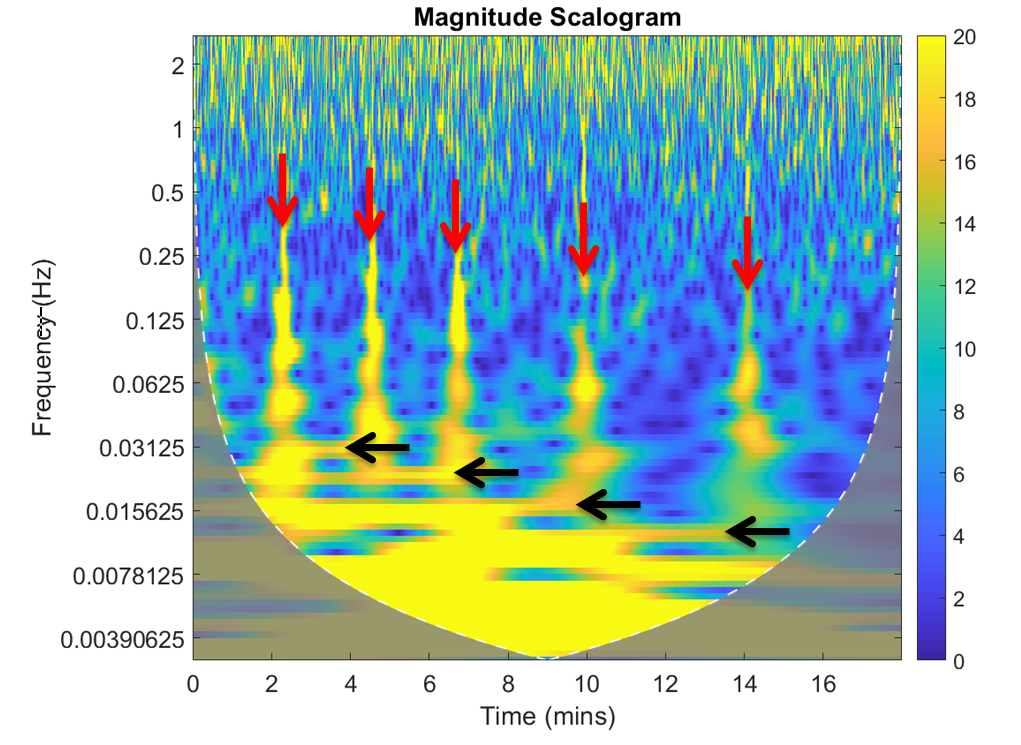
\includegraphics[width=0.7\textwidth]{figures/uncuffed_sub3_roi8_uncorr}
	\caption{Scalogram from the raw data from region eight in the uncuffed recording of subject 3.}
	\label{fig:scalogram_uncorr}
\end{figure}

Looking at the scalogram from the raw signal in \figref{fig:scalogram_uncorr} the jumps can easily be seen as the high bright spikes which represent the jumps in the signal. Five jumps that are indicated with the red arrows, are present in the scalogram at time points around 2.5, 4.5, 6.5, 10 and 14 minute time point in the signal. The jumps in the same signal shown in the time domain occur in the scalogram at the same time points. It is presumed that the corrected drift also is represented in the scalogram as low frequency content. Hereby different artifact components can be suspected to be included in the signal content. 

The artifact components of the raw signal can be sorted into three categories: 
\begin{itemize}
	\item Uniform white noise artifacts
    \item Drift artifacts within each interval
	\item Jumps artifacts
%	\item Generel drift in the signal
\end{itemize}

Uniform white noise artifacts is characterized by having the same magnitude in all frequencies. This artifact will therefore not affect the signal of interest, because it will have a flat power spectral density throughout the bandwidth of the frequencies, because the signal of the white noise are independent and evenly distributed \cite{hida2014}. 
The jumps in the signal is induces by the auto-adjustments from the camera described in \ref{sec:artifacts}. The drift artifacts can be seen as magnitudes in the scalogram as lower frequencies than the jumps. A frequency band leading up to a high spike occur with each jump indicated with black arrows arrow in \figref{fig:scalogram_uncorr}, indicating that the drift is not uniform between intervals.
The artifact components will be disturbing the presumed signal from the micro oscillations to get a representative cwt, because this signal can be hidden by the artifacts. The artifacts are not constant for each recording, why the correction of the signal has been implemented.

\begin{figure}[H]
	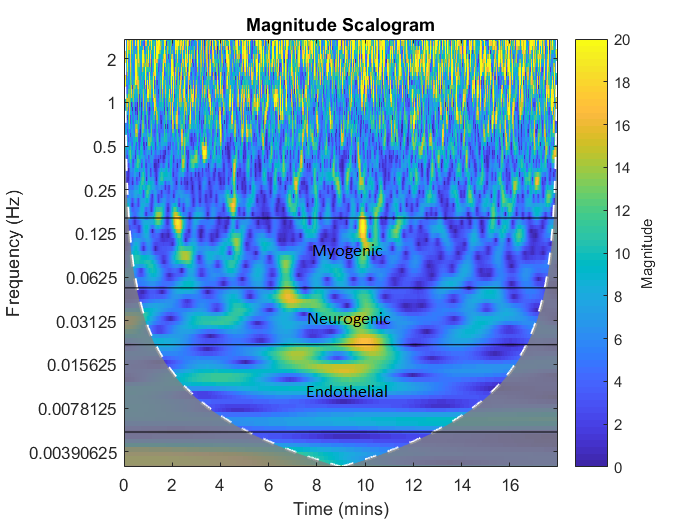
\includegraphics[width=0.7\textwidth]{figures/uncuffed_sub3_roi8_corr}
	\caption{Scalogram from the corrected data of region 8 in the uncuffed recording of subject 3, where a dampening of the spikes and  induced by the jumps has been achieved.}
	\label{fig:scalogram_corr}
\end{figure} 

After the correction of the signal, the energy has been reduced in the areas induced from the jumps and the drift. The scalogram is left with less energy overall as seen in \figref{fig:scalogram_corr}. %It can be discussed if the correction of the signal affects the signal of interest. 

The three frequency bands are divided by black lines in the scalogram seen in \figref{fig:scalogram_corr}.
To prepare the data for the statistical test, the average magnitude for each time period of each frequency band is first calculated by equation \ref{eq:W_avg}.
\begin{flalign}
W(n_{f})=\frac{1}{N} \sum_{n=1}^{N} W_n(n_{f})
\label{eq:W_avg}
\end{flalign}
Where N denotes the total number of elements in the frequency band, $W$ is the magnitude of the wavelet, $n_{f}$ is the respective frame and $n$ is the current element of the magnitude of the frequency band.

Then the mean of the average magnitude over the time period is calculated by equation \ref{eq:W_mean}
\begin{flalign}
	W_{mean}=\frac{1}{N_{f}} \sum_{n_f=1}^{N_{f}} W(n_{f})
	\label{eq:W_mean}
\end{flalign}
Where $W_{mean}$ denotes the mean value of the frequency band over the time period and $N_{f}$ is the total number of frames.
This gives a single value for the specific frequency band to use in the statistical test for comparison between the two conditions.